% ============================================================
% physio-placebo — meeting brief for an HCI conversation
% Compile: tectonic reports/hci_meeting_brief.tex
% ============================================================
\documentclass[11pt]{article}

\usepackage[a4paper,margin=0.82in]{geometry}
\usepackage{iftex}
\ifPDFTeX
  \usepackage[T1]{fontenc}
  \usepackage[utf8]{inputenc}
  \usepackage{lmodern}
\else
  \usepackage{fontspec}
\fi
\usepackage{microtype}
\usepackage{amsmath}
\usepackage{booktabs}
\usepackage{colortbl}
\usepackage{array}
\usepackage{tabularx}
\usepackage{ragged2e}
\usepackage{xcolor}
\usepackage{titlesec}
\usepackage{fancyhdr}
\usepackage{lastpage}
\usepackage{enumitem}
\usepackage{needspace}
\usepackage{graphicx}
\graphicspath{{figures/}}
\usepackage{caption}
\usepackage[hidelinks]{hyperref}

\captionsetup{
  font=small,
  labelfont={bf,color=Accent},
  textfont={color=AccentSoft},
  skip=3pt,
}

\definecolor{Accent}{HTML}{0F4C5C}
\definecolor{AccentSoft}{HTML}{1B6B7A}
\definecolor{RuleGray}{HTML}{B8C4C8}
\definecolor{TableHead}{HTML}{E8F1F3}
\definecolor{Ask}{HTML}{7A2E0E}
\definecolor{Ok}{HTML}{1F6B4A}
\definecolor{Muted}{HTML}{5C6B70}
\definecolor{BoxFill}{HTML}{F4F8F9}

\hypersetup{
  pdftitle={physio-placebo: meeting brief},
  pdfauthor={Shrijak Kumar},
  pdfsubject={Independent study briefing for an HCI conversation},
  linkcolor=Accent,
  urlcolor=AccentSoft,
}

\titleformat{\section}
  {\large\bfseries\color{Accent}}
  {\thesection}{0.65em}{}
\titlespacing*{\section}{0pt}{1.05em}{0.35em}
\titleformat{\subsection}
  {\normalsize\bfseries\color{AccentSoft}}
  {\thesubsection}{0.55em}{}
\titlespacing*{\subsection}{0pt}{0.75em}{0.22em}

\pagestyle{fancy}
\fancyhf{}
\renewcommand{\headrulewidth}{0.4pt}
\renewcommand{\footrulewidth}{0.3pt}
\fancyhead[L]{\small\color{AccentSoft} physio-placebo}
\fancyhead[R]{\small\color{AccentSoft} meeting brief\ \textbullet\ 22 Sep 2026}
\fancyfoot[L]{\small\color{Muted} Shrijak Kumar\ \textbullet\ Dr.\ Siddharth}
\fancyfoot[R]{\small\color{Muted} \thepage\ / \pageref{LastPage}}

\arrayrulecolor{Accent!55}
\setlength{\parindent}{0pt}
\setlength{\parskip}{0.42em}
\linespread{1.04}
\setlength{\emergencystretch}{2.2em}
\setlist[itemize]{leftmargin=1.15em,itemsep=0.12em,topsep=0.2em}
\setlist[enumerate]{leftmargin=1.2em,itemsep=0.12em,topsep=0.2em}
\newcolumntype{L}[1]{>{\RaggedRight\arraybackslash}p{#1}}
\newcolumntype{C}[1]{>{\centering\arraybackslash}p{#1}}
\newcolumntype{Y}{>{\RaggedRight\arraybackslash}X}

\newcommand{\say}[1]{{\color{Ask}\textbf{#1}}}

\begin{document}

{\large\scshape\color{AccentSoft} Independent study\ \textbullet\ reading brief\par}
\vspace{0.28em}
{\color{Accent}\hrule height 1.15pt}
\vspace{0.55em}
{\LARGE\bfseries\color{Accent} physio-placebo\par}
\vspace{0.15em}
{\large Is the model reading the wearable, or is the prompt doing the classifying?\par}
\vspace{0.45em}
{\color{Accent}\hrule height 1.15pt}
\vspace{0.6em}

\begin{tabular}{@{}L{3.15cm}L{12.4cm}@{}}
\textbf{Who} & Shrijak Kumar, independent study, Plaksha University \\
\textbf{Advisor} & Dr.\ Siddharth \\
\textbf{This note} & 22 September 2026. Weeks 1--6 are closed. Weeks 7--8 have not started. \\
\textbf{Pre-registration} & \url{https://osf.io/62r5t}\quad DOI 10.17605/OSF.IO/62R5T \\
\end{tabular}

\vspace{0.15em}
{\small\color{Muted}
Numbers below are the locked runs (seed 1337). Macro-F1 is the metric throughout.
A 95\% interval in brackets is a bootstrap over subjects, 1{,}000 resamples.
\par}

% ------------------------------------------------------------
\section{Open with this}

\noindent\fcolorbox{Accent}{BoxFill}{%
\begin{minipage}{\dimexpr\textwidth-2\fboxsep-2\fboxrule\relax}
\setlength{\parskip}{0.35em}
\vspace{0.35em}
{\small\color{AccentSoft}\scshape Read aloud, about one minute\par}
\vspace{0.15em}
I am checking a claim that is showing up in wearable and health-LLM papers: that a language model can tell stress or cognitive load from a sensor window. The tasks are ordinary lab tasks in HCI. WESAD is stress versus calm, from the ICMI wearable dataset, 15 people. MAUS is mental workload, easy versus hard n-back, 22 people, wrist PPG. CogWear is Stroop versus rest on an Empatica E4, 10 usable people.

Each example is a 60-second window from one person in one condition. Before any language model ran, I locked a classical floor on the same features. On WESAD, logistic regression reaches 0.92 macro-F1. The best language-model cell so far is 0.60, and a line plot of the same ECG scores at chance, about 0.41.

Those are real-signal numbers. The test that decides whether the model is using the physiology is still ahead: replace the recording with matched noise, with another person, or with an empty prompt, and see what accuracy is left. That comparison is pre-registered. It has not been run.
\vspace{0.2em}
\end{minipage}}

\vspace{0.55em}
{\small
\noindent\textbf{Six facts to keep in hand.}\par
\vspace{0.2em}
\begin{tabularx}{\textwidth}{@{}L{3.15cm}Y@{}}
\rowcolor{TableHead}
\textbf{Fact} & \textbf{Locked value} \\
\midrule
People & WESAD 15, MAUS 22, CogWear 10 usable of 11 \\
Windows & 1{,}042 / 1{,}086 / 114, each 60\,s, stride 30\,s, zero feature-NaN drops \\
Strong floor & WESAD logreg 0.918. MAUS 0.444 and CogWear 0.569 are weak \\
Best LLM so far & Qwen3-8B, WESAD, raw ECG averaged to 128 bins: 0.595 [0.550, 0.647] \\
Plots & Qwen2.5-VL at chance: WESAD 0.412, MAUS 0.400 \\
Not run yet & Surrogate ladder, adjective ablation, and the SDS score \\
\bottomrule
\end{tabularx}}

% ------------------------------------------------------------
\section{The question, in HCI terms}

Published prompting papers report that a language model can infer a state from wearable text. They rarely test whether that accuracy depends on the recording. This study runs the same kind of prompt under leave-one-subject-out, then replaces the recording and measures what remains.

The sharp part is the wording. A typical feature sentence says ``heart rate is elevated, stress-typical.'' The adjective can classify the window with no need to read the number. Week~9 strips those words, and also flips them, to see which one the model follows.

Three HCI constructs, three public lab datasets:

\begin{center}
{\small
\begin{tabularx}{\textwidth}{@{}L{2.15cm}L{3.5cm}Y@{}}
\rowcolor{TableHead}
\textbf{Dataset} & \textbf{Construct} & \textbf{Why it is in the study} \\
\midrule
WESAD & Stress vs non-stress & The public benchmark people in affective computing already know. Chest EDA and breathing give a linear model an easy win, so an LLM that skips the recording has a high score to miss. \\
\addlinespace
MAUS & Mental workload & n-back is a standard workload induction. Cardiac features alone are weak here, so a high LLM score would be hard to dismiss as an easy dataset. \\
\addlinespace
CogWear & Cognitive load & Stroop versus rest on a consumer wristband. Small, and the classical signal is barely above chance. Stops the paper being a single-dataset WESAD result. \\
\bottomrule
\end{tabularx}
}
\end{center}

The ground truth on this grid is the \textbf{experimental condition}: the person was in the TSST, in a 2-back block, or in the Stroop. It is the right label for ``did the sensor recover the protocol.'' It is a poor label for ``how stressed did they feel.'' Self-report appears only in a separate reproduction (PMData, below), which is not part of the WESAD / MAUS / CogWear grid.

No new participants. All three sets are already public.

% ------------------------------------------------------------
\section{Where the work stands}

\begin{center}
{\small
\begin{tabularx}{\textwidth}{@{}L{4.15cm}L{2.55cm}Y@{}}
\rowcolor{TableHead}
\textbf{Block} & \textbf{State} & \textbf{What is true} \\
\midrule
Data and features & Closed 16 Sep & Three loaders, frozen NeuroKit2 0.2.13, leakage tests \\
Classical floor & Closed 16 Sep & Locked before any LLM grid run \\
OSF and anchor & Closed 20 Sep & Registration public. MedAlpaca gap is large, and kept \\
Text prompts A and B & Closed 21 Sep & Qwen3-8B and Llama-3.1-8B, 11{,}916 scores, 0 failures \\
Plot prompts C & Closed 21 Sep & Qwen2.5-VL, 1{,}896 scores, 0 failures, both at chance \\
Surrogate ladder & Not started & Weeks 7--8. The ``is it the signal?'' test \\
Adjective ablation & Not started & Week 9. Strip or flip the adjectives \\
SDS report card & Not started & Week 10. The mid-semester result \\
\bottomrule
\end{tabularx}
}
\end{center}

Models that actually ran, on a Plaksha HTI RTX A6000, fp16, vLLM: \textbf{Qwen3-8B}, \textbf{Llama-3.1-8B-Instruct}, and \textbf{Qwen2.5-VL-7B-Instruct}. Scoring is one forward pass. The prediction is whichever of the tokens \texttt{A} or \texttt{B} has the higher log-probability. There is no free-written answer on the main grid.

The OSF page originally named GPT-4.1. A public update on the same registration records the switch. The API account was capped at 50 requests a day.

% ------------------------------------------------------------
\section{The datasets, in the form the code uses}

Every dataset is cut the same way. A window is 60 seconds. The next window starts 30 seconds later, so neighbors overlap by half. A window never crosses a condition boundary. If a sample inside a window is NaN, that window is dropped and counted. In the finished matrices, the drop count is zero, and every feature cell is finite.

Statistics resample \textbf{people}, not windows. Overlapping windows from one person are one subject.

\subsection{WESAD --- stress}

Schmidt et al., ICMI 2018. Public UCI release, 15 subjects: \texttt{S2}--\texttt{S11} and \texttt{S13}--\texttt{S17}. Lab protocol with a chest RespiBAN and a wrist Empatica E4. Conditions in the file are baseline, amusement, stress (Trier Social Stress Test: speech and mental arithmetic), and meditation.

\textbf{Binary task used here.} Stress (protocol code 2) versus non-stress, where non-stress is baseline plus amusement (codes 1 and 3). Meditation and the transient codes are left out. Amusement is a real affective state; in this task it sits in the negative class. The model is asked ``stress or not,'' and is not asked to name amusement.

\textbf{What one window contains.} Five synchronized channels, float samples:

\begin{center}
{\small
\begin{tabularx}{\textwidth}{@{}L{1.7cm}L{2.55cm}L{1.45cm}L{1.7cm}Y@{}}
\rowcolor{TableHead}
\textbf{Channel} & \textbf{Sensor} & \textbf{Rate} & \textbf{Samples} & \textbf{Role in this study} \\
\midrule
\texttt{ecg} & Chest ECG & 700\,Hz & 42{,}000 & Raw-series prompt, plot, and all 8 HRV features \\
\texttt{eda} & Chest EDA & 700\,Hz & 42{,}000 & 7 skin-conductance features \\
\texttt{resp} & Chest Resp & 700\,Hz & 42{,}000 & 3 breath features \\
\texttt{bvp} & Wrist BVP & 64\,Hz & 3{,}840 & Stored in the window file \\
\texttt{eda\_wrist} & Wrist EDA & 4\,Hz & 240 & Stored in the window file \\
\bottomrule
\end{tabularx}
}
\end{center}

Accelerometer, EMG, and temperature are in the original zip and are not loaded. The language-model prompts and the feature vector use the three chest channels. Wrist BVP and wrist EDA are kept in the window file and are outside the locked feature plan.

\textbf{Counts.} 1{,}042 windows. 731 non-stress, 311 stress (about 70 / 30). Prompt-development subjects, chosen by seed and then held out of every reported LLM number: \texttt{S2} and \texttt{S8} (136 windows). Evaluation: 13 people, 906 windows.

\textbf{Feature vector.} 18 numbers, identical for the logistic regression and for the verbalized prompt:
8 HRV from the chest ECG (mean NN interval, SDNN, RMSSD, pNN50, mean heart rate, LF power, HF power, LF/HF),
7 EDA from chest conductance after a cvxEDA split (tonic mean and spread, phasic spread, skin-conductance response count and mean amplitude, raw level mean and spread),
3 respiration (breath-rate mean and spread, mean breath amplitude).
LF power on a 60\,s window is at the edge of what that band can resolve. That limit is documented and shared with a lot of short-window HRV work.

\subsection{MAUS --- mental workload}

IEEE DataPort, DOI 10.21227/q4td-yd35. 22 subjects: \texttt{002}--\texttt{006}, \texttt{008}, \texttt{010}--\texttt{025}. Wrist PixArt PPG during n-back. The authors' files also contain a chest ECG and a fingertip PPG; this study follows the wrist PPG, which is the channel their baseline code treats as the wrist stream.

\textbf{Binary task.} Low workload = 0-back. High workload = 2-back and 3-back. Trials 1 and 6 are 0-back, trials 2 and 4 are 2-back, trials 3 and 5 are 3-back. Resting recordings are excluded, so the contrast is difficulty inside the task. There is no 1-back column in this layout.

\textbf{Sampling.} 100\,Hz for subjects 002--006, and 102.5\,Hz for the rest, matching the authors' baseline code. A 60\,s window is therefore 6{,}000 samples or 6{,}150 samples of one PPG channel. Subjects 002--006 contribute 54 windows each; the others contribute 48 each.

\textbf{Counts.} 1{,}086 windows. 362 low, 724 high (one third / two thirds). Held out of LLM eval: subjects \texttt{015} and \texttt{023} (96 windows). Evaluation: 20 people, 990 windows.

\textbf{Feature vector.} 8 HRV features only, from the wrist PPG peaks. No EDA and no respiration in the locked MAUS matrix. That is why the classical floor is weak: the positive class has to be read from a wrist pulse wave.

\subsection{CogWear --- Stroop}

PhysioNet database \texttt{consumer-grade-wearables}, version 1.0.0, pilot cohort only (subject ids 0--10). The survey-gamification cohort is a different protocol and is excluded. Task: resting baseline versus a Stroop cognitive-load session. Sensors in this study: Empatica E4 blood-volume pulse at 64\,Hz and EDA at 4\,Hz. Muse EEG, a Samsung band, and temperature files exist upstream and are outside the locked spec.

\textbf{One window.} BVP: 3{,}840 samples. EDA: 240 samples. The two clocks are trimmed to their overlap before windowing, and the sample spacing is checked against the nominal rate.

\textbf{Exclusion.} Pilot subject 3 has no \texttt{cognitive\_load/empatica\_eda.csv} on PhysioNet (checked against the published SHA256 list). The missing-channel rule drops that person before any model runs. Usable cohort: 10.

\textbf{Counts.} 114 windows. 39 baseline, 75 Stroop. About a handful of windows per person, which is why every CogWear interval later is wide. Held out: subjects 4 and 8. Evaluation: 8 people, 90 windows.

\textbf{Feature vector.} 15 numbers: the same 8 HRV features, here from wrist BVP, plus the same 7 EDA features. No respiration.

\subsection{Side dataset, used once: PMData}

The fidelity anchor is a different problem, on purpose. Health-LLM (Kim et al., CHIL 2024) predicts self-reported stress on a 1--5 scale from PMData: 16 people, Fitbit daily summaries (steps, calories, resting heart rate, sleep) plus a mood rating, written out as text. It is not a raw waveform, and it is not scored with macro-F1. It exists so the study can show one published number next to a re-run, before interpreting our own grid.

% ------------------------------------------------------------
\section{How a window is shown to the model}

Three views of the same 60\,s window. Each cell keeps the view that won a small prompt search, then that choice is frozen.

\begin{figure}[!ht]
\centering
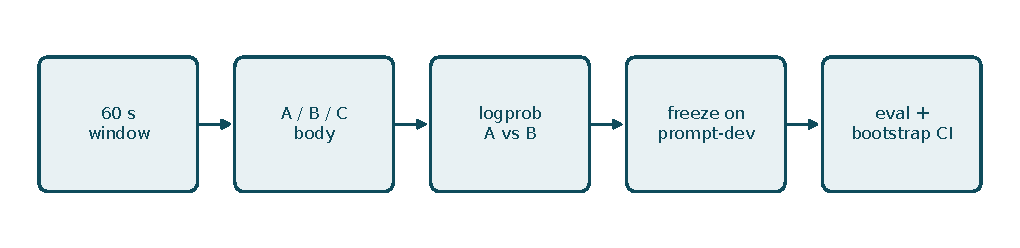
\includegraphics[width=\textwidth]{fig_methods.pdf}
\caption{One scored item. The window becomes text or a plot. The model returns probabilities for the tokens A and B. The reported number uses evaluation subjects only.}
\end{figure}

\textbf{Paradigm A --- raw numbers.} The primary channel only: WESAD chest ECG, MAUS wrist PPG, CogWear wrist BVP. Two compressions, both reported, because 42{,}000 ECG samples do not fit a prompt and there is no uniquely correct downsample:
\begin{itemize}
  \item \textbf{uniform stride,} 256 kept samples;
  \item \textbf{bin mean,} 128 non-overlapping averages.
\end{itemize}
The winning WESAD cell is bin-mean. The prompt body looks like this (middle values omitted):

{\small\ttfamily
ecg fs=700 Hz n=128 scheme=bin\_mean:\\
0.04024 0.005173 -0.01352 -0.01912 0.03245 \ldots\ -0.04705 -0.00251 -0.06615
\par}

\textbf{Paradigm B --- sentences.} The 18 / 15 / 8 features, rendered with the original adjectives. ``High'' is above the median of the \emph{other} subjects in that fold, so the test window does not define its own threshold. Four of the eighteen WESAD sentences, from a real window:

{\small\ttfamily
eda\_tonic\_mean is reduced (0.7358), calmer-typical.\\
hrv\_mean\_hr is elevated (89.28), stress-typical.\\
hrv\_sdnn is reduced (41.18), stress-typical.\\
hrv\_rmssd is reduced (17.7), stress-typical.
\par}

The words ``stress-typical'' and ``calmer-typical'' are intentional. They are the leak Week~9 is built to measure. The numbers in the current B results still sit next to those words.

\textbf{Paradigm C --- a line plot.} Matplotlib, fixed size (6.4\,in by 2.4\,in, 100\,dpi), black line, time in seconds on the x-axis. Same window, same PNG bytes. No subject id and no class name on the axes. Primary channel only. WESAD ECG and MAUS PPG. CogWear has no plot cell. The model is Qwen2.5-VL-7B-Instruct.

\begin{figure}[!ht]
\centering
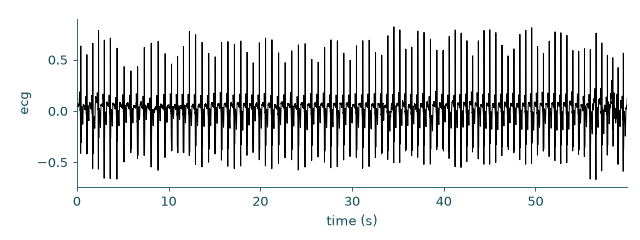
\includegraphics[width=0.88\textwidth]{fig_input_c.png}
\caption{Paradigm C for one WESAD ECG window. This image is the entire signal input.}
\end{figure}

\textbf{Label tokens.} Single letters, so they stay one token:
WESAD A = non-stress, B = stress;
MAUS A = low-workload, B = high-workload;
CogWear A = baseline, B = stroop.

\textbf{Prompt search, then freeze.} Three wordings (instruction, clinical, minimal) times zero-shot or four-shot. The winner is chosen on two people only, then locked. Four-shot examples come from those two people and from nobody else. The search is not repeated after a result looks bad. Frozen winners for the best WESAD cell: clinical wording, zero-shot, bin-mean ECG. Plot cells: instruction wording, four-shot, on both WESAD and MAUS.

% ------------------------------------------------------------
\section{Classical floor, chance, and the score we have not computed}

The floor uses the same feature matrix the verbalizer uses, byte for byte. L2 logistic regression and a depth-3 tree. Strict leave-one-subject-out. Seed 1337. Chance is two numbers: the majority-class macro-F1, and a 1{,}000-permutation floor that shuffles labels inside each subject.

\begin{center}
{\small
\begin{tabular}{@{}lccccc@{}}
\toprule
\rowcolor{TableHead}
\textbf{Dataset} & \textbf{Logreg} & \textbf{Tree} & \textbf{Majority} & \textbf{Perm.\ p95} & \textbf{Read} \\
\midrule
WESAD ($n{=}15$) & 0.918 & 0.848 & 0.412 & 0.433 & Strong \\
MAUS ($n{=}22$) & 0.444 & 0.482 & 0.400 & 0.413 & Weak \\
CogWear ($n{=}10$) & 0.569 & 0.560 & 0.397 & 0.541 & Barely there \\
\bottomrule
\end{tabular}
}
\end{center}
{\small\color{Muted}
The permutation column is the 95th percentile of logistic regression under within-subject label shuffles. MAUS's tree (0.482) clears its own permutation p95 (0.453). CogWear's tree (0.560) does not clear its own (0.566). Per-subject logreg on WESAD is $0.913 \pm 0.107$.
\par}

\textbf{Why majority is about 0.40 and not 0.50.} Macro-F1 averages the two classes. A classifier that always says ``non-stress'' scores 0 on the stress class, so the average lands near 0.41 on WESAD even though accuracy would look like 70\%. The dashed line on the figures is that majority macro-F1. The permutation p95 is the stricter ``could this feature set do this by luck'' line.

\textbf{SDS, defined, not yet a number.} When the surrogates exist,
\[
\mathrm{SDS}
=
\frac{M_{\mathrm{real}}-M_{\mathrm{surrogate}}}{M_{\mathrm{real}}-M_{\mathrm{chance}}}.
\]
$M$ is pooled leave-one-subject-out macro-F1. If a cell's real-signal margin over the permutation floor has a bootstrap interval that includes zero, SDS is left undefined and only the raw gap is reported. MAUS and CogWear are the cells where that gate is expected to bind. Pre-registered predictions: SDS below 0.3 for raw series and for plots; the verbalized condition loses more than half its above-chance margin when the adjectives are neutralized; mis-signed adjectives flip more than 40\% of items.

The surrogate list, identical for every cell once it is run: Gaussian noise matched to the global mean and variance; IAAFT phase-randomized surrogates; another subject's recording with the condition link broken; a flatline; the prompt with the signal deleted. A label-preserving subject swap is reported beside those and is not treated as a null. A logistic regression is run on every surrogate so the ledger shows how much class information each one still holds.

% ------------------------------------------------------------
\section{What the real-signal runs actually did}

The classical floor uses every subject. The LLM tables hold out the two prompt-development subjects. On WESAD the floor is 0.92 and the best LLM cell is 0.60. Holding out two people does not close a gap that size.

\begin{figure}[!ht]
\centering
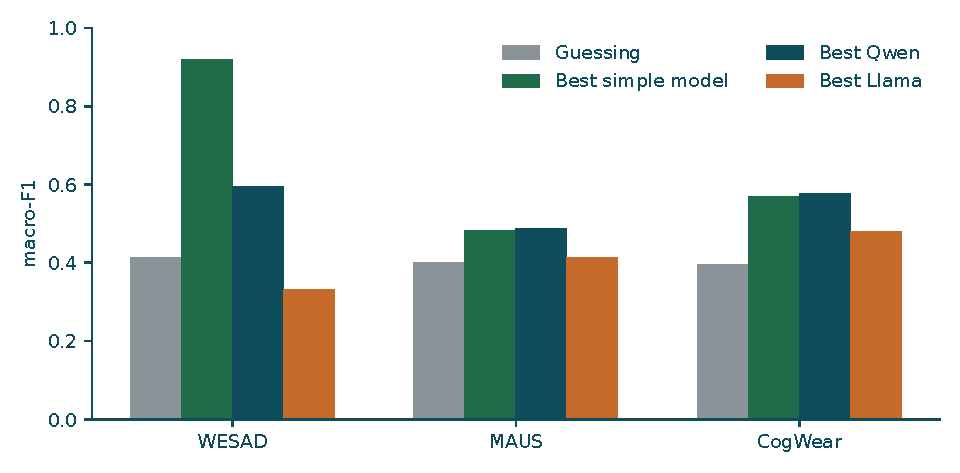
\includegraphics[width=\textwidth]{fig_floors_vs_llm.pdf}
\caption{Locked classical floor against the best real-signal A/B cell of each model. WESAD is the only dataset where the linear model is far above majority. Each LLM bar is the best of that model's three A/B cells.}
\end{figure}

\Needspace{11\baselineskip}
\subsection{Paradigms A and B}

Evaluation subjects only. Intervals are subject bootstraps.

\begin{center}
{\small
\begin{tabular}{@{}llcc@{}}
\toprule
\rowcolor{TableHead}
\textbf{Dataset} & \textbf{Cell} & \textbf{Qwen3-8B} & \textbf{Llama-3.1-8B} \\
\midrule
WESAD & A, stride 256 & 0.427 [0.392, 0.465] & 0.333 [0.301, 0.370] \\
WESAD & A, bin-mean 128 & \textbf{0.595 [0.550, 0.647]} & 0.230 [0.227, 0.233] \\
WESAD & B, verbalizer & 0.584 [0.462, 0.699] & 0.283 [0.247, 0.324] \\
MAUS & A, stride 256 & 0.467 [0.436, 0.499] & 0.413 [0.403, 0.426] \\
MAUS & A, bin-mean 128 & 0.483 [0.452, 0.516] & 0.400 [0.400, 0.400] \\
MAUS & B, verbalizer & 0.487 [0.439, 0.531] & 0.400 [0.400, 0.400] \\
CogWear & A, stride 256 & 0.576 [0.443, 0.689] & 0.404 [0.392, 0.417] \\
CogWear & A, bin-mean 128 & 0.396 [0.380, 0.411] & 0.440 [0.399, 0.495] \\
CogWear & B, verbalizer & 0.475 [0.393, 0.504] & 0.479 [0.375, 0.640] \\
\bottomrule
\end{tabular}
}
\end{center}

How to say this table out loud. On WESAD, Qwen clears the majority line (0.41) in the bin-mean cell and in the verbalizer, and remains far below logistic regression (0.92). The verbalizer interval is wide: 0.46 to 0.70. Llama's best WESAD cells sit below the majority line. On MAUS, two Llama cells are exactly 0.400 with a zero-width interval: the model emitted one class for every window of every evaluation subject. That is a constant prediction, and the run did not crash. CogWear intervals are wide because the eval set is 90 windows from 8 people. A point estimate of 0.58 there is not a ranking.

\begin{figure}[!ht]
\centering
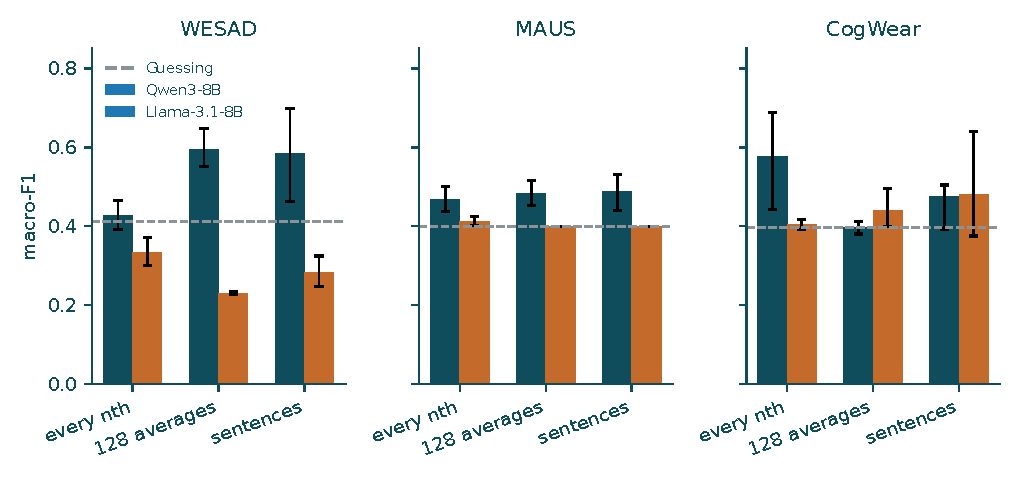
\includegraphics[width=\textwidth]{fig_ab_grid.pdf}
\caption{Real-signal A and B. Dashed line: majority-class macro-F1. Qwen is the stronger of the two text models on WESAD and MAUS.}
\end{figure}

\subsection{Paradigm C, and the Health-LLM re-run}

\begin{center}
{\small
\begin{tabular}{@{}lccc@{}}
\toprule
\rowcolor{TableHead}
\textbf{Dataset} & \textbf{Prompt} & \textbf{macro-F1 [95\% CI]} & \textbf{Eval windows} \\
\midrule
WESAD & instruction, 4-shot & 0.412 [0.410, 0.414] & 906 \\
MAUS & instruction, 4-shot & 0.400 [0.399, 0.400] & 990 \\
\bottomrule
\end{tabular}
}
\end{center}

Both sit on the majority line. The intervals are tiny because the vision model almost always emits one class. That matches the pre-registered expectation that a plot prompt would carry little of the signal. The prompts were not retuned after this result.

The Health-LLM anchor, separate data and metric: zero-shot MedAlpaca-7B on PMData stress, three seeds. Paper: MAE $0.76 \pm 0.1$. This re-run: MAE $\mathbf{2.689 \pm 0.038}$ (seeds 2.714, 2.645, 2.708), 6 parse failures out of 897. The completions mostly say ``out of 5'' or ``out of 10,'' and the locked scorer reads the first number, so it records 5 or 10. The scorer was not changed to close the gap. Their released code does not run as published; the patches required to execute it are written down. On their own label distribution, always answering 3 has MAE about 0.43, which beats most of the LLM cells in their Table~16. They do not report that baseline.

% ------------------------------------------------------------
\section{If the conversation goes there}

\say{So did the model read the physiology?}
On the real signal, a linear model on standard features is still well ahead on WESAD, and the plot model is at chance. That is suggestive. It is not the surrogate test. The honest sentence is: we have measured real-signal performance, and we have not yet measured how much of it survives when the recording is replaced.

\say{Why these sets, instead of a new user study?}
A new TSST is an ethics and logistics project. These three are public, they are the tasks HCI already uses (stress, n-back, Stroop), and they disagree with each other in a useful way: one strong classical signal, two weak ones. The design needs that spread. WESAD alone would be a near-ceiling dataset. CogWear alone would be too small to conclude anything.

\say{Is chance 50\%?}
For accuracy, the majority rate is the constant-classifier baseline: about 70\% on WESAD, about 67\% on MAUS, about 66\% on CogWear. The reported metric is macro-F1, which gives the missed class a vote. The constant classifier then scores about 0.40. Both numbers are in the locked floor files. Quote macro-F1 against 0.40, and mention accuracy only if asked for the class balance.

\say{Aren't overlapping windows leaking?}
They overlap in time, inside one person and one condition. They never contain two people's data, and they never mix two labels. The interval is a bootstrap over subjects. A window is not treated as an independent sample.

\say{Why is logistic regression so much better on WESAD?}
Chest EDA and respiration in a scripted social-stress protocol are highly separable. Tonic skin conductance alone is known to carry a lot of this contrast. The language model, in the raw-series cell, sees a downsampled ECG and does not see those EDA features. In the verbalizer cell it does see them, as sentences that also contain the words ``stress-typical,'' and it still lands near 0.58 with a wide interval. Both facts can be said in the same breath.

\say{Then is 0.60 a success?}
It is the best LLM cell, it clears WESAD majority, and it is far below the floor that uses the same people and a simple model. Llama on that same bin-mean input scores 0.23, which is worse than always saying non-stress. Model identity is doing a lot of work. I would not describe 0.60 as the model understanding stress.

\say{What is the verbalizer point, in one example?}
``\texttt{hrv\_mean\_hr} is elevated (89.28), stress-typical.'' A reader can follow either the number or the last two words. Week~9 writes the same sentence with the number and a percentile only, and a third version that says ``reduced'' when the value is high. Those runs are the paper. They are not in the current tables.

\say{What would change your mind?}
A raw-series or plot cell whose accuracy collapses when the recording is replaced by spectrum-matched noise or by nothing. That is a high SDS, and it is the opposite of the pre-registered prediction. Equally, a verbalizer that keeps its margin after the adjectives are removed. Either result is publishable. The registration is what makes the negative one publishable too.

\say{Is 10 to 22 people enough?}
It is the public cohort, and it is small. CogWear's intervals already show it. The bootstrap is over subjects because a thousand windows from 10 people are not a thousand independent tests. I would rather show a wide interval than borrow precision from overlapping windows.

\say{What did the Health-LLM re-run mean?}
Their headline cell did not come back. The gap is about +1.9 MAE, and it is reported as the result. Part of the mechanism is visible: the model emits a denominator (``out of 5'') and a first-number parser records the denominator. I am not treating our grid as a verdict on their paper. I am treating the failed reproduction as a reason to be slow about any new LLM-versus-wearable number, including ours.

\say{Which channel should I mention if they ask ``what is the input''?}
For a raw prompt or a plot: one channel, chest ECG on WESAD, wrist PPG on MAUS, wrist BVP on CogWear, compressed or drawn. For the verbalizer and the classical floor: the feature vector, 18 / 8 / 15 numbers, from chest ECG+EDA+respiration, wrist PPG, or wrist BVP+EDA respectively.

% ------------------------------------------------------------
\section{What is left, and the sentence to end on}

Next, in order, and not started: the five surrogates plus the separate label-preserving swap, on every frozen cell, with a classical model run on each surrogate; then the adjective ablation on Paradigm~B; then one SDS report card. SensorLM's captioning templates are vendored as an optional fourth verbalizer. They are Google's wording, Apache-2.0, and they are waiting on a yes or no. SensorLM itself has no public weights, so it is not a model in this study.

\vspace{0.25em}
\noindent\fcolorbox{Accent}{BoxFill}{%
\begin{minipage}{\dimexpr\textwidth-2\fboxsep-2\fboxrule\relax}
\vspace{0.4em}
\textbf{Close.} The datasets are public lab inductions of stress, workload, and Stroop. The unit is a 60-second window. A linear model already solves WESAD. The language models, given numbers, sentences, or a plot, do not match that floor, and the plot model is at chance. Whether any of the remaining accuracy is the physiology is the pre-registered experiment, and it is the part still in front of me.
\vspace{0.35em}
\end{minipage}}

\vspace{0.8em}
{\color{Accent}\hrule height 0.6pt}
\vspace{0.35em}
{\small\color{AccentSoft}
Sources for every figure and table: locked floors under \texttt{results/classical\_floor/}, eval grids under \texttt{results/eval\_grid/}, and the week log in \texttt{PROGRESS.md}. Weeks 1--6 tagged done on 21 September 2026. This note does not change the filed OSF text.
\par}

\end{document}
